\chapter{Beta and double beta decay}
Beta decay is a nuclear transition in which a nucleus $(Z, A)$ converts into an isobar $(Z \pm 1, A)$ through the weak interaction, with the emission of an electron or positron and the corresponding (anti)neutrino, as anticipated in Chapter~\ref{chapter:nuIntro}. The single-beta decay process can be written as
\begin{equation}
    \label{eq:single-beta-decay}
    (Z, A) \longrightarrow (Z+1, A) + e^- + \overline{\nu}_e \qquad \text{or} \qquad 
    (Z, A) \longrightarrow (Z-1, A) + e^+ + \nu_e,
\end{equation}
depending on whether a neutron ($\beta^-$) or a proton ($\beta^+$) undergoes the weak transition. Enrico Fermi described this process in 1934~\cite{Fermi1934} by introducing a point-like, four-fermion contact interaction Hamiltonian
\begin{equation}
    H_F = G_F \left( \overline{\psi}_p \gamma^\mu \psi_n \right)\left( \overline{\psi}_e \gamma_\mu \psi_\nu \right) + \text{h.c.}
\end{equation} 
with $G_F$ the Fermi coupling constant, later reinterpreted within the \ac{SM} as the low-energy, effective limit of the \ac{CC} interaction (Eq.~\ref{eq:SM-neutrino-lagrangian}) where a virtual $W$ boson mediates, at the quark level, the $d \to u$ or $u \to d$ transitions. The process is allowed whenever it is energetically favourable, i.e. whenever its $Q$-value, given by the mass difference between the parent and daughter atoms, is positive. It is precisely this energy balance, together with nuclear pairing effects, that determines which nuclei undergo ordinary $\beta$ decay and which ones are instead only accessible through the second-order process of double-$\beta$ decay, discussed further in this Chapter.

\section{Two-neutrino double beta decay (\texorpdfstring{$2\nu\boldsymbol{\beta}\boldsymbol{\beta}$}{2vbb})}
\label{sec:2nubetabeta}
Double beta decay is a second-order weak interaction process in which a nucleus $(Z, A)$ decays directly into one of its isobars $(Z\pm2, A)$, changing its charge by two units while leaving the mass number unchanged. First proposed in 1935 by Maria Goeppert-Mayer~\cite{firstDoubleBeta}, it can be seen as the double counterpart of single-$\beta$ decay. Just as the latter comes in the $\beta^-$, $\beta^+$ and \ac{EC} variants, double beta decay with the emission of two neutrinos, $2\nu\beta\beta$, can proceed through four different modes: $\beta^-\beta^-$, $\beta^+\beta^+$, $\beta^+$\ac{EC} and \ac{EC}\ac{EC}, where in the last two the nucleus captures one or two electrons from the atomic shells. All of them perfectly conserve the lepton number and are fully accommodated within the \ac{SM}. They are summarised in Table~\ref{tab:bb-modes}.

\begin{table}[H]
    \centering
    \begin{tabular}{ll}
        \toprule
        \textbf{decay mode} & $\boldsymbol{2\nu}$ \textbf{channel} \\
        \midrule
        $\beta^-\beta^-$ & $(Z,A) \to (Z+2,A) + 2e^- + 2\overline{\nu}_e$ \\
        $\beta^+\beta^+$ & $(Z,A) \to (Z-2,A) + 2e^+ + 2\nu_e$ \\
        $\beta^+$\ac{EC} & $e^-_\text{b} + (Z,A) \to (Z-2,A) + e^+ + 2\nu_e$ \\
        \ac{EC}\ac{EC} & $2e^-_\text{b} + (Z,A) \to (Z-2,A) + 2\nu_e$ \\
        \bottomrule
    \end{tabular}
    \caption{Possible modes of $2\nu\beta\beta$ decay. $e^-_\text{b}$ denotes an electron captured from the atomic shell.}
    \label{tab:bb-modes}
\end{table}

The energy conditions differ from mode to mode. Working with atomic masses, the $\beta^-\beta^-$ decay only requires $M(Z,A) > M(Z+2,A)$. For the modes that decrease the nuclear charge, the mass difference $M(Z,A) - M(Z-2,A)$ must instead exceed $2m_ec^2 \simeq 1022$~keV for $\beta^+$\ac{EC} and $4m_ec^2 \simeq 2044$~keV for $\beta^+\beta^+$, since each emitted positron costs $2m_ec^2$, while the \ac{EC}\ac{EC} mode has no such penalty. In addition, the Coulomb repulsion between the nucleus and the positron further suppresses positron emission. As a result, the modes involving $\beta^+$ and \ac{EC} generally have low effective $Q$-values and rates much smaller than $\beta^-\beta^-$, and are usually neglected. In principle, each of these modes could also occur without the emission of neutrinos, a lepton-number-violating process discussed in Section~\ref{sec:0nubetabeta}. 

Seeing that this work focuses on ${}^{76}$Ge double-beta decay, in what follows $\beta\beta$ refers to the $\beta^-\beta^-$ mode detailed in the first row of Table~\ref{tab:bb-modes}.

At the microscopic level, the process occurs through two simultaneous, virtual single-$\beta$ transitions, as illustrated by the two weak vertices in the Feynman diagram of Figure~\ref{fig:2nu_feynman}.

\begin{figure}[H]
    \centering
    \begin{center}
\begin{tikzpicture}[
    thick,
    % Stile per le linee dei fermioni (linea con freccia a metà)
    fermion/.style={draw=black, postaction={decorate},
        decoration={markings, mark=at position 0.55 with {\arrow{latex}}}},
    % Stile per i bosoni W (linea ondulata)
    boson/.style={draw=black, decorate,
        decoration={snake, amplitude=1mm, segment length=3.5mm}},
    % Stile per i vertici dei nucleoni (i cerchi grigi)
    blob/.style={circle, draw=black, fill=gray!30, minimum size=6mm, inner sep=0pt}
]

% ---------------- NUCLEONE SUPERIORE ----------------
% Frecce esterne n e p
\draw[fermion] (-4.5, 2) node[left, font=\Large] {n} -- (-3, 2);
\draw[fermion] (3, 2) -- (4.5, 2) node[right, font=\Large] {p};

% Le 3 linee dei quark all'interno (tra i due blob)
\draw[fermion] (-3, 2.15) -- (3, 2.15);
\draw[fermion] (-3, 2.0) -- (3, 2.0);
\draw[fermion] (-3, 1.85) -- (3, 1.85);

% Bosone W- 
\draw[boson] (0, 1.85) -- (1.5, 0.8);
\node[font=\Large] at (0.4, 1.2) {$W^-$};

% Elettrone e antineutrino 
% (Nota: la linea del neutrino è disegnata da destra a sinistra per invertire la freccia)
\draw[fermion] (1.5, 0.8) -- (3.5, 1.3) node[right, font=\Large] {$e^-$};
\draw[fermion] (3.5, 0.3) node[right, font=\Large] {$\overline{\nu}_e$} -- (1.5, 0.8);


% ---------------- NUCLEONE INFERIORE ----------------
% Frecce esterne n e p
\draw[fermion] (-4.5, -2) node[left, font=\Large] {n} -- (-3, -2);
\draw[fermion] (3, -2) -- (4.5, -2) node[right, font=\Large] {p};

% Le 3 linee dei quark all'interno (tra i due blob)
\draw[fermion] (-3, -1.85) -- (3, -1.85);
\draw[fermion] (-3, -2.0) -- (3, -2.0);
\draw[fermion] (-3, -2.15) -- (3, -2.15);

% Bosone W- 
\draw[boson] (0, -1.85) -- (1.5, -0.8);
\node[font=\Large] at (0.4, -1.2) {$W^-$};

% Elettrone e antineutrino
\draw[fermion] (1.5, -0.8) -- (3.5, -0.3) node[right, font=\Large] {$e^-$};
\draw[fermion] (3.5, -1.3) node[right, font=\Large] {$\overline{\nu}_e$} -- (1.5, -0.8);


% --- DISEGNO I BLOB ---
% (Disegnati per ultimi così coprono perfettamente le estremità delle linee)
\node[blob] at (-3, 2) {};
\node[blob] at (3, 2) {};
\node[blob] at (-3, -2) {};
\node[blob] at (3, -2) {};

\end{tikzpicture}
\end{center}
    \caption{Feynman diagram of $2\nu\beta\beta$. The process proceeds via the exchange of two virtual $W^-$ bosons, resulting in the simultaneous emission of two electrons and two electron antineutrinos.}
    \label{fig:2nu_feynman}
\end{figure}

\begin{wrapfigure}{l}{0.52\textwidth}%[H]
    \centering
    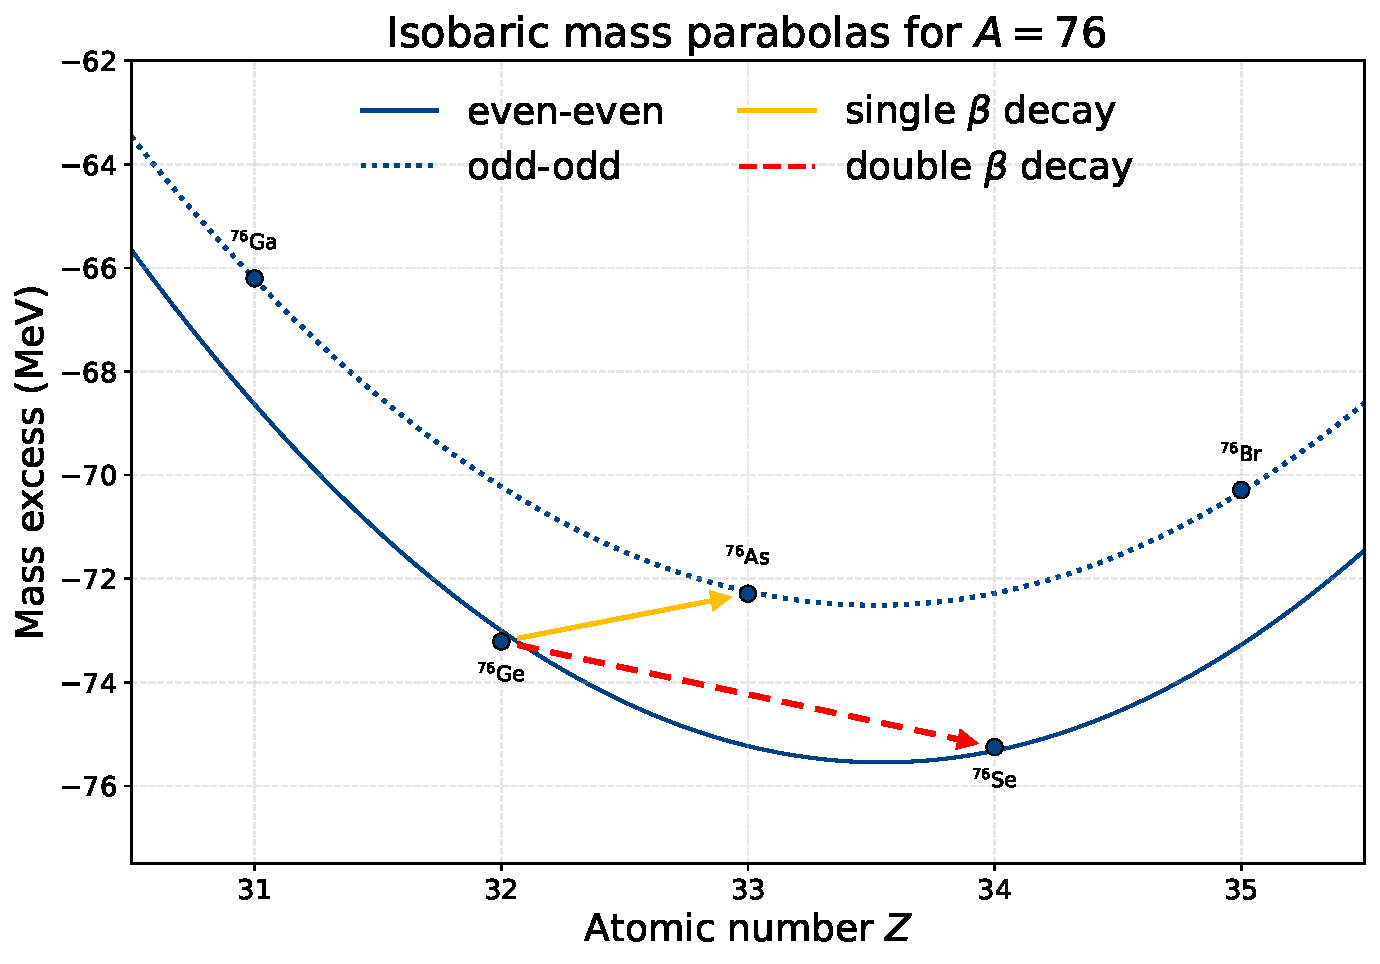
\includegraphics[width=\linewidth]{figures/mass_parabola_A76.pdf}
    \caption{Mass parabolas for $A=76$ isobars. A detailed description is given in the text. Custom plot with data taken from \cite{AME2020-masses} and \cite{Ge76-Qvalue}.}
    \label{fig:doublebeta-parabola}
\end{wrapfigure}
For a nucleus to undergo such a rare decay, the standard single-$\beta$ decay to the intermediate isobar $(Z+1, A)$ must be energetically forbidden or heavily suppressed. This kinematic condition naturally arises in even-even nuclei due to the nuclear pairing interaction, which binds them more tightly than their odd-odd neighbours. As a consequence, while the direct transition $(Z, A) \to (Z+1, A)$ is blocked, the target state $(Z+2, A)$ still sits at a lower energy level, effectively opening the double-$\beta$ channel. 
This energy landscape is visualised using mass parabolas, as shown in Figure~\ref{fig:doublebeta-parabola} for the case of ${}^{76}\text{Ge}$, where the even-even and odd-odd mass parabolas are shown with a continuous and dashed line, respectively. The double-beta transition of ${}^{76}\text{Ge}$ is highlighted in red, while the yellow lines represent ordinary single-$\beta$ decays. The intermediate odd-odd state acts as a virtual state in the quantum mechanical transition and is never physically populated.

Because $2\nu\beta\beta$ is a second-order process in the weak coupling, its decay rate is massively suppressed compared to ordinary $\beta$ decay, resulting in extremely long half-lives of the order of $T_{1/2}^{2\nu} \sim 10^{19}$--$10^{24}$~years, depending on the isotope.

Unlike the neutrinoless mode, $2\nu\beta\beta$ does not require any new physics beyond the \ac{SM} and has been experimentally observed in about 10 different even-even isotopes. Nuclei such as ${}^{76}\text{Ge}$ are of particular relevance in modern physics, as they also represent the most promising candidates in the search for neutrinoless double beta decay, a process that violates lepton number by two units and is discussed in detail in Section~\ref{sec:0nubetabeta}.

\section{Neutrinoless double beta decay (\texorpdfstring{$0\nu\boldsymbol{\beta}\boldsymbol{\beta}$}{0vbb})}
\label{sec:0nubetabeta}

In Section~\ref{sec:2nubetabeta}, $2\nu\beta\beta$ was introduced as a rare second-order weak process, allowed by the \ac{SM} because it conserves lepton number. Neutrinoless double-$\beta$ decay ($0\nu\beta\beta$) differs from it by a single, but crucial, feature: no (anti)neutrino is present in the final state, so that the processes of Table~\ref{tab:bb-modes} are to be rewritten as in Table~\ref{tab:0nubb-modes}.


\begin{table}[H]
    \centering
    \begin{tabular}{ll}
        \toprule
        \textbf{decay mode} & $\boldsymbol{0\nu}$ \textbf{channel} \\
        \midrule
        $\beta^-\beta^-$ & $(Z,A) \to (Z+2,A) + 2e^-$\\
        $\beta^+\beta^+$ & $(Z,A) \to (Z-2,A) + 2e^+$\\
        $\beta^+$\ac{EC} & $e^-_\text{b} + (Z,A) \to (Z-2,A) + e^+$ \\
        \ac{EC}\ac{EC} & $2e^-_\text{b} + (Z,A) \to (Z-2,A)$\\
        \bottomrule
    \end{tabular}
    \caption{Possible modes of $0\nu\beta\beta$ decay. $e^-_\text{b}$ denotes an electron captured from the atomic shell.}
    \label{tab:0nubb-modes}
\end{table}


This implies a violation of lepton number by two units ($\Delta L=2$), which is forbidden in the \ac{SM}. Its observation would therefore be a clear signal of physics beyond the \ac{SM}, with several implications. Since the decay can be mediated by different mechanisms (e.g.\ the exchange of a light Majorana neutrino, of heavy particles or right-handed currents~\cite{review-0nu-2015}), these implications can be divided into two groups: those that do not depend on the mediating mechanism, and those that hold only under specific assumptions on it.

\begin{enumerate}
\item \textbf{model-independent consequences}:
\begin{itemize}
    \item \textit{matter creation}: it would be the first laboratory observation of a process that produces matter without producing the corresponding antimatter.
    \item \textit{violation of lepton number and of $B-L$}: since the baryon number $B$ is not affected by the decay, a $\Delta L = 2$ process also violates $B-L$. This would be the first experimental evidence that such a symmetry, which is only accidental in the \ac{SM} and has no theoretical reason to be exact, is broken in nature.
    \item \textit{Majorana nature of neutrinos}: whatever the underlying mechanism, an observed $0\nu\beta\beta$ decay implies that neutrinos can convert into antineutrinos, hence that they are Majorana particles.
\end{itemize}

\item \textbf{model-dependent consequences}: if the decay is dominated by the exchange of a light Majorana neutrino, the measured half-life can be translated into a value of the effective Majorana mass $m_{\beta\beta}$ (see Eq.~\ref{eq:half-life_0nubb} below), which gives access to:
\begin{itemize}
    \item \textit{absolute neutrino mass scale}: oscillation experiments are sensitive only to mass-squared differences, while combining $m_{\beta\beta}$ with direct measurements from single $\beta$ decay and with cosmological data allows one to constrain the individual mass eigenvalues (central and right panels of Fig.~\ref{fig:mbb_allowed});
    \item \textit{mass ordering}: comparing $m_{\beta\beta}$ with the regions allowed for the normal and inverted ordering (Fig.~\ref{fig:mbb_allowed}), the ordering could be established. In the inverted case $m_{\beta\beta}$ is bounded from below, while in the normal one it can vanish. If $m_{\beta\beta}$ falls where the two regions overlap, the ordering can be established only by combining it with an independent measurement of the mass scale, through $m_\beta$ or $\Sigma$.
\end{itemize}
\end{enumerate} 

The model-independent results are also relevant for cosmology. The Universe appears to contain only matter, and the \ac{SM} cannot account for the observed matter-antimatter asymmetry: although it contains sources of $CP$ and baryon-number violation, two of the conditions identified by Sakharov~\cite{sakharov}, they are too weak to generate it. A new source of violation of global symmetries is therefore needed, and leptogenesis models provide it: a lepton asymmetry is generated through lepton-number-violating processes and then partially converted into a baryon asymmetry. Observing $0\nu\beta\beta$ would support this class of scenarios~\cite{morella}.


As established earlier, this work centres on ${}^{76}\text{Ge}$. Hereafter, we consider exclusively the light-neutrino exchange channel for its neutrinoless decay, formulated in Eq.~\ref{eq:0nu-beta-beta} and represented in Figure~\ref{fig:0nubetabeta-diagram}.

\begin{equation}
    \label{eq:0nu-beta-beta}
    (Z, A) \longrightarrow (Z+2, A) + 2e^-
\end{equation} 

\begin{figure}[H]
    \centering
    \begin{center}
\begin{tikzpicture}[
    thick,
    % Stile per le linee dei fermioni (linea con freccia a metà)
    fermion/.style={draw=black, postaction={decorate},
        decoration={markings, mark=at position 0.55 with {\arrow{latex}}}},
    % Stile per i bosoni W (linea ondulata)
    boson/.style={draw=black, decorate,
        decoration={snake, amplitude=1mm, segment length=3.5mm}},
    % Stile per la massa di Majorana (la X al centro)
    cross/.style={cross out, draw=black, thick, minimum size=6pt, inner sep=0pt},
    % Stile per i vertici dei nucleoni (i cerchi grigi)
    blob/.style={circle, draw=black, fill=gray!30, minimum size=6mm, inner sep=0pt}
]

% ---------------- NUCLEONE SUPERIORE ----------------
\draw[fermion] (-4.5, 2) node[left, font=\Large] {n} -- (-3, 2);
\draw[fermion] (3, 2) -- (4.5, 2) node[right, font=\Large] {p};

\draw[fermion] (-3, 2.15) -- (3, 2.15);
\draw[fermion] (-3, 2.0) -- (3, 2.0);
\draw[fermion] (-3, 1.85) -- (3, 1.85);

% ---------------- NUCLEONE INFERIORE ----------------
\draw[fermion] (-4.5, -2) node[left, font=\Large] {n} -- (-3, -2);
\draw[fermion] (3, -2) -- (4.5, -2) node[right, font=\Large] {p};

\draw[fermion] (-3, -1.85) -- (3, -1.85);
\draw[fermion] (-3, -2.0) -- (3, -2.0);
\draw[fermion] (-3, -2.15) -- (3, -2.15);

% --- DISEGNO I BLOB ---
\node[blob] at (-3, 2) {};
\node[blob] at (3, 2) {};
\node[blob] at (-3, -2) {};
\node[blob] at (3, -2) {};

% ---------------- SCAMBIO INTERNO ----------------
% Bosoni W
\draw[boson] (-0.5, 1.85) -- (0.5, 0.7);
\draw[boson] (-0.5, -1.85) -- (0.5, -0.7);

% Neutrino di Majorana (dritto, senza freccia, con la X)
\draw (0.5, 0.7) -- (0.5, -0.7);
\node[cross, label={[font=\Large]right:{$\nu_M$}}] at (0.5, 0) {};

% Elettroni uscenti
\draw[fermion] (0.5, 0.7) -- (3.5, 1.3) node[right, font=\Large] {$e^-$};
\draw[fermion] (0.5, -0.7) -- (3.5, -1.3) node[right, font=\Large] {$e^-$};

\end{tikzpicture}
\end{center}
    \caption{Feynman diagram for neutrinoless double $\beta$-decay. The Majorana coupling of the neutrino with its own antineutrino (see Figure~\ref{fig:feynman-massCouplings}) is shown.}
    \label{fig:0nubetabeta-diagram}
\end{figure}


\begin{wrapfigure}{l}{0.52\textwidth}%[H]
    \centering
    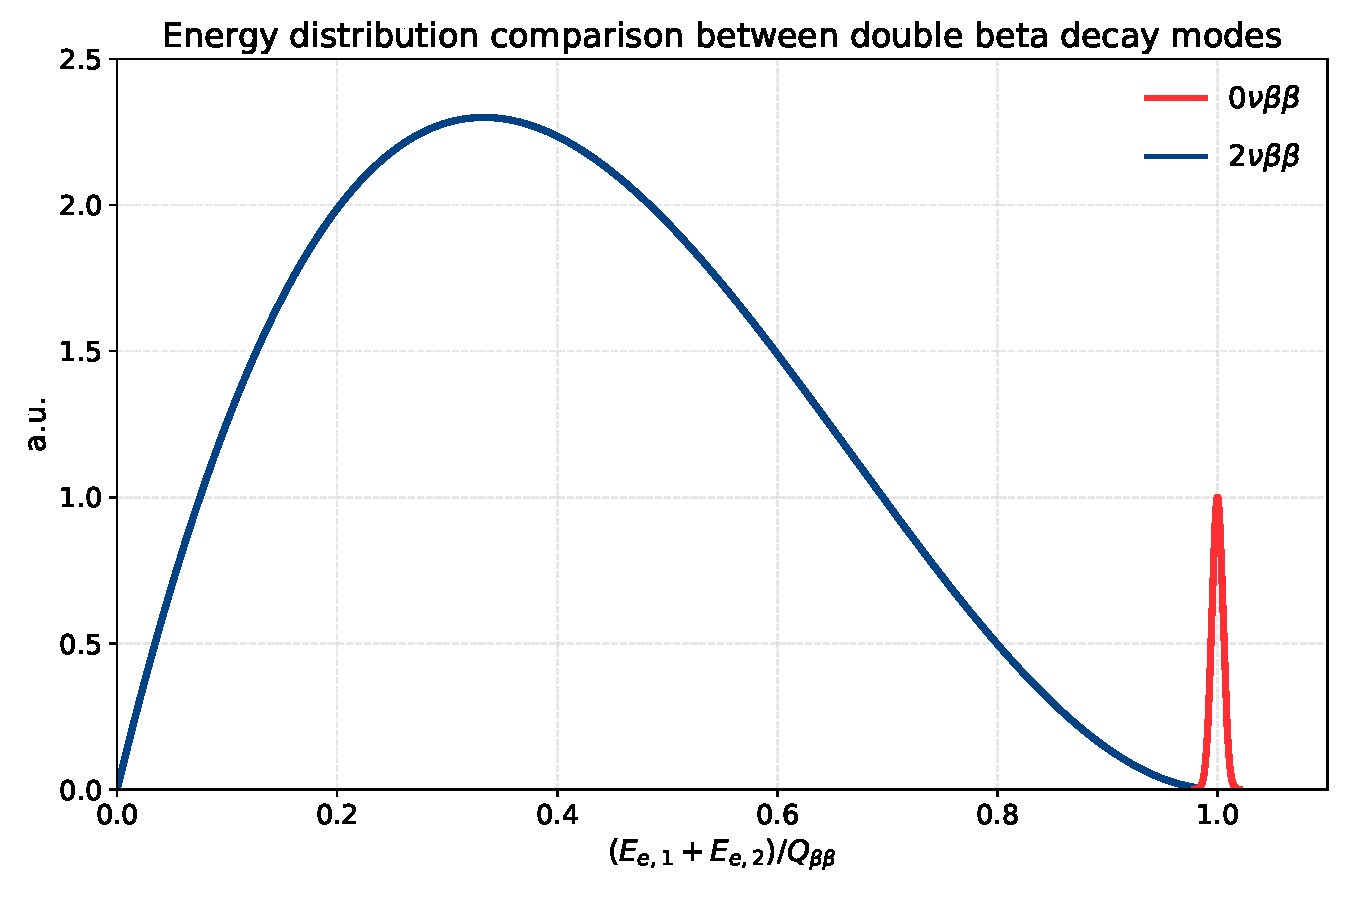
\includegraphics[width=\linewidth]{figures/0nu_vs_2nu.pdf}
    \caption{Schematic representation of the energy distribution for the products in $2\nu\beta\beta$ and $0\nu\beta\beta$ decay modes. The description is given in the text.}
    \label{fig:Qvalue-2nu0nu}
\end{wrapfigure}
From an experimental point of view, $0\nu\beta\beta$ can be distinguished from the more common $2\nu\beta\beta$ decay by analysing the energy spectrum of the two emitted electrons. Specifically, in $0\nu\beta\beta$ decay, the electrons are produced with energies $E_{e, 1}$ and $E_{e, 2}$ that satisfy
\begin{equation*}
    E_{e, 1} + E_{e, 2} + E_{\text{nuc}} = Q_{\beta\beta} = M(Z, A) - M(Z+2, A)
\end{equation*}
where $M(Z, A)$ and $M(Z+2, A)$ are the atomic masses of the parent and daughter atoms, respectively. Since the energy of the recoiling nucleus is negligible, the sum of the electron energies equals the $Q$-value of the transition, i.e. $E_{e, 1} + E_{e, 2} = Q_{\beta\beta}$. Conversely, in standard $2\nu\beta\beta$ decay part of the energy is carried away by the two antineutrinos, so the summed electron energy has a continuous spectrum that extends up to $Q_{\beta\beta}$, with a maximum around one third of $Q_{\beta\beta}$ and very few events close to the endpoint. Fig.~\ref{fig:Qvalue-2nu0nu} shows this continuous spectrum in blue for the $2\nu\beta\beta$ process and the monoenergetic peak\footnote{The signal has ideally a Dirac delta signature but is represented here as a very narrow Gaussian because what would be eventually observed is limited by detector resolution.} at $Q_{\beta\beta}$ for $0\nu\beta\beta$ in red.

If neutrinos are indeed Majorana particles and the standard mechanism for $0\nu\beta\beta$ decay is mediated by the exchange of a light Majorana neutrino, the decay rate, usually expressed in terms of the half-life $T_{1/2}^{0\nu}$, is given by:
\begin{equation}
    \label{eq:half-life_0nubb}
    (T_{1/2}^{0\nu})^{-1} = G_{0\nu}(Q_{\beta\beta}, Z) \left| \mathcal{M}_{0\nu} \right|^2 \left( \frac{m_{\beta\beta}}{m_e} \right)^2
\end{equation}
where $G_{0\nu}(Q_{\beta\beta}, Z)$ is the phase space factor, which depends on the $Q$-value and on the atomic number $Z$, $\mathcal{M}_{0\nu}$ is the nuclear matrix element, $m_e$ is the electron mass, and $m_{\beta\beta} = \big|\sum_{i=1}^{3} U_{ei}^2\, m_i\big|$ denotes the effective Majorana mass. The latter depends on the elements of the first row of $U_\text{PMNS}^\text{Maj}$, including the Majorana phases, and on the neutrino mass eigenvalues; through $m_{\beta\beta}$, the decay rate is therefore also sensitive to the \ac{NMO}.

Using the parametrisation of Eqs.~\ref{eq:Upmns-majorana} and~\ref{eq:Upmns-total}, the effective Majorana mass can be written explicitly as
\begin{equation}
  m_{\beta\beta} = \left| c_{12}^2 c_{13}^2\, m_1 + s_{12}^2 c_{13}^2\, m_2\, e^{i\alpha_{21}} + s_{13}^2\, m_3\, e^{i(\alpha_{31}-2\delta)} \right| .
  \label{eq:mbb_explicit}
\end{equation}
Mixing angles and mass-squared differences are measured by oscillation experiments, but $m_{\beta\beta}$ also depends on three quantities they cannot access: the two Majorana phases and the absolute mass scale. For a given mass scale, letting the phases vary between the values that maximise and minimise $m_{\beta\beta}$ defines its allowed range. The mass scale can be expressed through the lightest neutrino mass $m_\text{light}$ ($m_1$ for normal and $m_3$ for inverted ordering), through the effective electron-neutrino mass measured in single $\beta$ decay, $m_\beta = \big(\sum_i |U_{ei}|^2 m_i^2\big)^{1/2}$, or through the sum of the masses constrained by cosmology, $\Sigma = \sum_i m_i$. The resulting regions are shown in Fig.~\ref{fig:mbb_allowed}.

At large mass scales the three neutrinos are quasi-degenerate and the two orderings overlap, while at lower values they separate. In the inverted ordering the two dominant terms of Eq.~\ref{eq:mbb_explicit} cannot cancel, since $\cos 2\theta_{12} \neq 0$, so $m_{\beta\beta}$ is bounded from below at about 18~meV~\cite{plot-esperiments_and_exposures}: next-generation experiments such as LEGEND-1000 aim to probe this whole region. In the normal ordering, instead, the three terms can cancel for $m_\text{light}$ of a few meV, and $m_{\beta\beta}$ can be arbitrarily small. Oscillation data also set a minimum value of $\Sigma$, about 59~meV for normal and 100~meV for inverted ordering, which is where the two regions start in the right panel.

\begin{figure}[H]
  \centering
  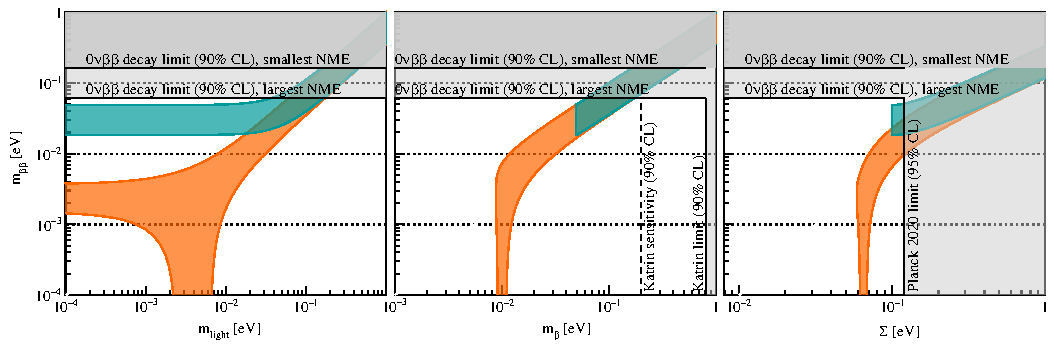
\includegraphics[width=\textwidth]{figures/mbb_NO_IO_Agostini2023.pdf}
  \caption[Allowed range of $m_{\beta\beta}$ as a function of $m_\text{light}$, $m_\beta$ and $\Sigma$]{%
  Range of $m_{\beta\beta}$ allowed by light Majorana neutrino exchange as a function of the lightest neutrino mass $m_\text{light}$ (left), of the effective electron-neutrino mass $m_\beta$ (centre) and of the sum of the neutrino masses $\Sigma$ (right), for normal (orange) and inverted (teal) ordering. The oscillation parameters are fixed to their central values, so the width of each region is due only to the unknown Majorana phases. Grey areas are excluded by $0\nu\beta\beta$ searches (KamLAND-Zen, 2016; the two horizontal lines correspond to the largest and smallest nuclear matrix element), by KATRIN (central panel) and by Planck (right panel); the dashed line in the central panel is the KATRIN design sensitivity. Limits are those available in 2023 (see text for updates). Figure taken from~\cite{plot-esperiments_and_exposures}.}
  \label{fig:mbb_allowed}
\end{figure}

The limits shown in Fig.~\ref{fig:mbb_allowed} reflect the status in 2023 and have since improved: KamLAND-Zen now sets $T_{1/2}^{0\nu} > 3.8\times10^{26}$~yr (Table~\ref{tab:0nubb-limits}), while the KATRIN and cosmological bounds have become $m_\beta < 0.45$~eV~\cite{katrin2025} and $\Sigma < 0.064$~eV~\cite{desi2025}, as anticipated in Section~\ref{subsec:NMO}. The cosmological bound, obtained by combining DESI DR2 and CMB data within $\Lambda$CDM, is already in tension with the minimum value allowed by oscillations, and relaxes to 0.163~eV if the dark energy equation of state is allowed to evolve~\cite{desi2025}.

Experimentally, observing $0\nu\beta\beta$ decay requires identifying a tiny, mono-energetic signal at $Q_{\beta\beta}$, so the choice of the best isotope to search for such a rare decay is the first issue to face, since it involves background suppression and energy resolution considerations, but also the limited time for which an experiment can be run. These considerations translate into a series of criteria for choosing a suitable isotope, which restrict the choice to elements with high isotopic abundance, a good compatibility with detection techniques and a sufficiently high $Q_{\beta\beta}$. The $Q$-values of the candidate isotopes span from about $2$~MeV up to a few MeV, a range where the dominant background is the environmental radioactivity of the natural ${}^{232}$Th and ${}^{238}$U decay chains, together with cosmic rays. Since the intensity of this background decreases with increasing energy, isotopes with a high enough $Q_{\beta\beta}$ are preferred, so that the region of interest lies where the background is lowest. To give an idea of the energy scale, natural $\gamma$ radioactivity extends up to the $2615$~keV line of ${}^{208}$Tl, the $\beta$ decay of ${}^{214}$Bi, from the ${}^{238}$U chain, reaches $3270$~keV, and $\alpha$ decays are even more energetic, around $5$~MeV (e.g. $5.3$~MeV for ${}^{210}$Po)~\cite{review-0nu-2015}.

Thus, the commonly studied isotopes are the ones listed in Table~\ref{tab:isotopes-for-0nu}, together with their isotopic abundance and $Q_{\beta\beta}$ values. ${}^{76}$Ge is an exception among them, since its $Q_{\beta\beta} = 2039$~keV lies in a region where natural $\gamma$ radioactivity is still present, which is in principle a limitation for background reduction. It is nevertheless one of the most studied isotopes, thanks to the excellent energy resolution and radiopurity of high-purity germanium detectors, in which the source coincides with the detector.

\begin{table}[H]
    \centering
    \begin{tabular}{lcc}
        \toprule
        Isotope & Isotopic abundance (\%) & $Q_{\beta\beta}$ [keV] \\
        \midrule
        ${}^{48}\text{Ca}$  & 0.187 & 4263 \\
        ${}^{76}\text{Ge}$  & 7.8   & 2039 \\
        ${}^{82}\text{Se}$  & 9.2   & 2998 \\
        ${}^{96}\text{Zr}$  & 2.8   & 3348 \\
        ${}^{100}\text{Mo}$ & 9.6   & 3035 \\
        ${}^{116}\text{Cd}$ & 7.6   & 2813 \\
        ${}^{130}\text{Te}$ & 34.08 & 2527 \\
        ${}^{136}\text{Xe}$ & 8.9   & 2459 \\
        ${}^{150}\text{Nd}$ & 5.6   & 3371 \\
        \bottomrule
    \end{tabular}
    \caption{Candidate isotopes for $0\nu\beta\beta$ search: isotopic abundance and $Q_{\beta\beta}$ value. Data are taken from \cite{review-0nu-2015}.}
    \label{tab:isotopes-for-0nu}
\end{table}

If a $0\nu\beta\beta$ signal is detected, its half-life can be experimentally evaluated as 
\begin{equation}
    \label{eq:half-life_0nubb_exp}
    T_{1/2}^{0\nu} = \ln(2) \cdot T \cdot \varepsilon \cdot \frac{N_{\beta\beta}}{N_\text{peak}}
\end{equation}
where $T$ is the measuring time, $\varepsilon$ is the detection efficiency, $N_{\beta\beta}$ is the number of $\beta\beta$-decaying nuclei under observation and $N_\text{peak}$ is the number of observed decays in the region of interest. If no peak is detected, the sensitivity of a given experiment is expressed in terms of a detector \textit{figure of merit} $S^{0\nu}$, i.e. the half-life corresponding to the maximum signal that could be hidden by the background fluctuations $n_{B}$. From Eq.~\ref{eq:half-life_0nubb_exp}, the sensitivity can be written as
\begin{equation}
    \label{eq:sensitivity-0nu}
    \begin{aligned}
        S^{0\nu} &= \ln 2 \cdot T \cdot \varepsilon \cdot \frac{N_{\beta\beta}}{n_\sigma \cdot n_B} \\
                 &= \ln 2 \cdot \varepsilon \cdot \frac{1}{n_\sigma} \cdot \frac{x\,\eta\,N_A}{\mathcal{M}_A} \cdot \sqrt{\frac{M \cdot T}{B \cdot \Delta E}},
    \end{aligned}
\end{equation}
where $n_\sigma$ is the confidence level in units of standard deviations and $n_B = \sqrt{B \cdot M \cdot T \cdot \Delta E}$ is the fluctuation of the number of background events in the region of interest~\cite{review-0nu-2015}. The exposure $M \cdot T$ is the product of detector mass and measuring time, $B$ is the background index, i.e. the background rate per unit mass, energy and time, and $\Delta E$ is the energy resolution (FWHM) at $Q_{\beta\beta}$. Finally, the second line follows from writing $N_{\beta\beta} = x\,\eta\,N_A\,M/\mathcal{M}_A$, where $x$ is the stoichiometric multiplicity of the candidate element in the compound, $\eta$ its isotopic abundance, $N_A$ Avogadro's number and $\mathcal{M}_A$ the molar mass of the compound.

This formula dictates the design of modern experiments: to maximise sensitivity, one must increase the exposure while minimising both the background level and the energy resolution. Specifically, a poor energy resolution causes the continuous tail of the standard $2\nu\beta\beta$ decay to smear into the $0\nu\beta\beta$ region of interest, creating an irreducible background.


\section{Experiments currently searching for \texorpdfstring{$0\nu\boldsymbol{\beta}\boldsymbol{\beta}$}{0nu beta beta} decay}
\label{sec:0nubb-experiments}
The experimental approach to $0\nu\beta\beta$ searches is based on the development of a detection technique able to balance good energy resolution, very low background and large isotope mass. Up to now, experiments in this field rely on two different techniques: calorimetric detectors, in which the source is embedded inside the detector volume itself, and detectors exploiting an external source~\cite{review-0nu-2015}. 

The best limits obtained so far for each candidate isotope are reported in Table~\ref{tab:0nubb-limits}~\cite{PDG:2026}, while the experiments currently running or planned, together with their expected sensitivities, are summarised in Fig.~\ref{fig:experiments-and-sensitivities-0nubb}.
\begin{table}[H]
    \centering
    \begin{tabular}{llc}
        \toprule
        Isotope & Experiment & $T_{1/2}^{0\nu}$ limit [yr] \\
        \midrule
        ${}^{48}\text{Ca}$  & CaF$_2$ scintillators     & $> 5.8 \times 10^{22}$ \\
        ${}^{76}\text{Ge}$  & GERDA + MJD + LEGEND-200  & $> 1.9 \times 10^{26}$ \\
        ${}^{82}\text{Se}$  & CUPID-0                   & $> 4.6 \times 10^{24}$ \\
        ${}^{96}\text{Zr}$  & NEMO-3                    & $> 9.2 \times 10^{21}$ \\
        ${}^{100}\text{Mo}$ & AMoRE-I                   & $> 2.9 \times 10^{24}$ \\
        ${}^{116}\text{Cd}$ & AURORA                    & $> 2.2 \times 10^{23}$ \\
        ${}^{130}\text{Te}$ & CUORE                     & $> 3.5 \times 10^{25}$ \\
        ${}^{136}\text{Xe}$ & KamLAND-Zen               & $> 3.8 \times 10^{26}$ \\
        ${}^{150}\text{Nd}$ & NEMO-3                    & $> 2.0 \times 10^{22}$ \\
        \bottomrule
    \end{tabular}
    \caption{Best current lower limits (90\% CL) on the $0\nu\beta\beta$ half-life for each candidate isotope \cite{PDG:2026}.}
    \label{tab:0nubb-limits}
\end{table}

\begin{figure}[H]
    \centering
    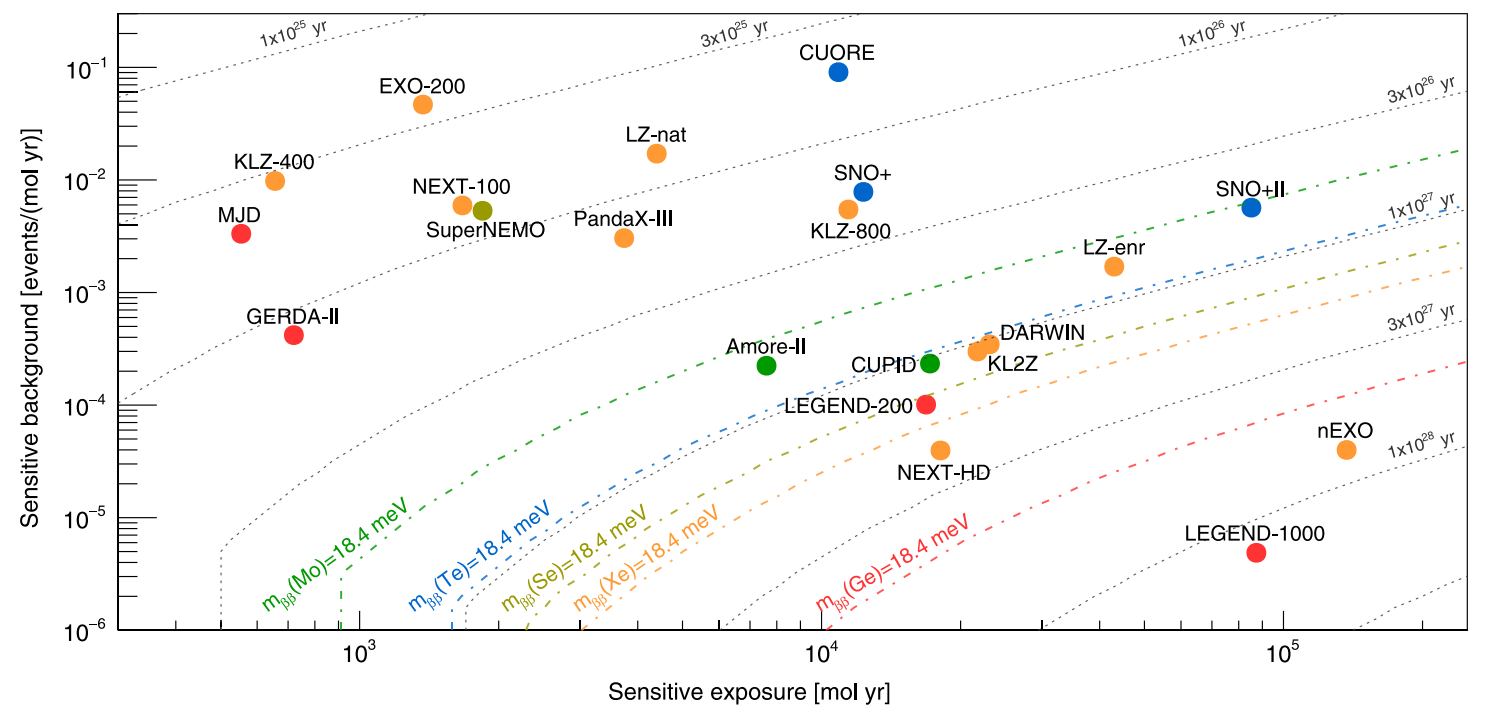
\includegraphics[width=\textwidth]{figures/experiments_and_sensitivities.png}
    \caption{Overview of the experiments searching for $0\nu\beta\beta$ decays with related sensitive exposures and backgrounds. Experiments marked in green exploit ${}^{100}$Mo, those in yellow use ${}^{136}$Xe, the blue ones employ ${}^{130}$Te, SuperNEMO is the only one using ${}^{82}$Se and finally red experiments exploit ${}^{76}$Ge. Plot taken from \cite{plot-esperiments_and_exposures}.}
    \label{fig:experiments-and-sensitivities-0nubb}
\end{figure}